

\documentclass[a4paper, 12pt]{article}
\usepackage[UTF8]{ctex}
\title{实验报告}
\author{23020007067 李子昊}
\date{\today}
\usepackage{fontawesome}
\usepackage{setspace}
\usepackage{color}    
\usepackage{float}
\usepackage{graphicx}
\usepackage[left=2cm,right=2cm,top=2cm,bottom=2cm,head=1cm,headsep=0.5cm,foot=1cm]{geometry}
\usepackage{hyperref}
\usepackage{indentfirst}
\hypersetup{hidelinks,
	colorlinks=true,
	allcolors=black,
	pdfstartview=Fit,
	breaklinks=true}
    
\begin{document}
\maketitle

\pagenumbering{roman}
\large \tableofcontents
\newpage
\pagenumbering{arabic}

\section{课后练习}
 \subsection{{\color{red}shell练习内容}}
 {\noindent 1.阅读 man ls ,然后使用 ls 命令进行如下操作:
\\
\\
\indent -所有文件(包括隐藏文件)
\vspace{-10pt}
\begin{figure}[H]
  \centering
  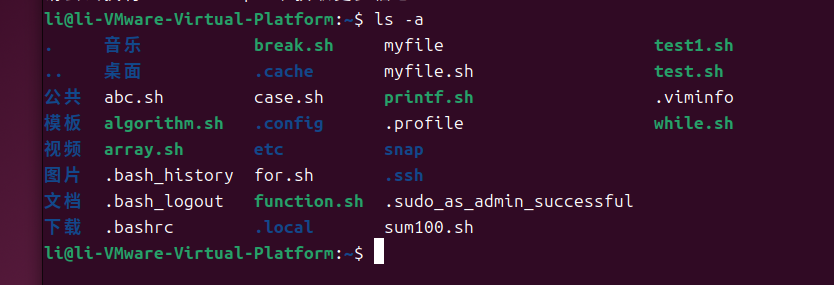
\includegraphics[width=1\textwidth]{屏幕截图 2024-09-05 133654.png}
  \caption{ls -a}
    \end{figure}
    
\indent -文件打印以人类可以理解的格式输出 
\vspace{-10pt}
\begin{figure}[H]
  \centering
  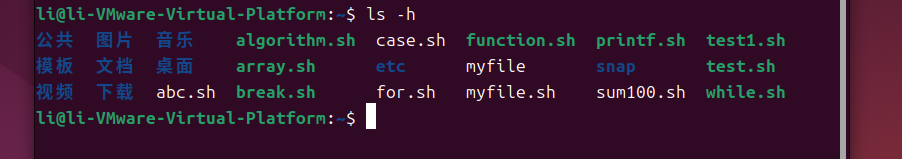
\includegraphics[width=1\textwidth]{屏幕截图 2024-09-05 133743.png}
  \caption{ls -t}
    \end{figure}
    
\indent -文件以最近访问顺序排序
\vspace{-10pt}
\begin{figure}[H]
  \centering
  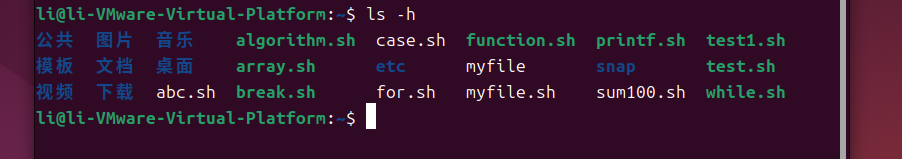
\includegraphics[width=1\textwidth]{屏幕截图 2024-09-05 133743.png}
  \caption{ls -t}
    \end{figure}
 \clearpage   
\indent -以彩色文本显示输出结果}
\vspace{-10pt}
\begin{figure}[H]
  \centering
  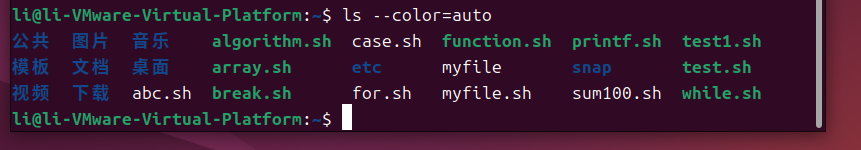
\includegraphics[width=1\textwidth]{屏幕截图 2024-09-05 133926.png}
  \caption{ls --color=auto}
    \end{figure}

\\
\noindent {2.编写两个 bash 函数 marco 和 polo 执行下面的操作。 每当你执行 marco 时,当前的工作目录应当以某种形式保存,当执行 polo 时,无论现在处在什么目录下,都应当 cd 回到当时执行 marco 的目录。 为了方便 debug,你可以把代码写在单独的文件 marco.sh 中,并通过 source marco.sh 命令,(重新)加载函数。}
\vspace{-10pt}
\begin{figure}[H]
  \centering
  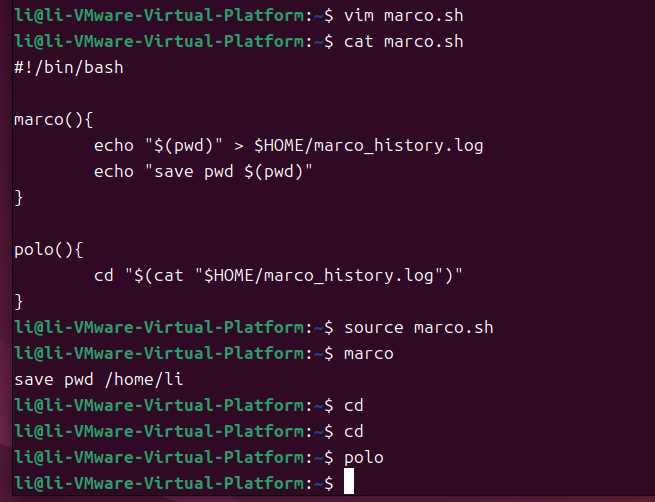
\includegraphics[width=1\textwidth]{屏幕截图 2024-09-05 135356.png}
  \caption{vim编译内容和shell操作指令}
    \end{figure}
\\
\newpage
\noindent {3.假设您有一个命令,它很少出错。因此为了在出错时能够对其进行调试,需要花费大量的时间重现错误并捕获输出。 编写一段 bash 脚本,运行如下的脚本直到它出错,将它的标准输出和标准错误流记录到文件,并在最后输出所有内容。 加分项:报告脚本在失败前共运行了多少次。}
\vspace{-10pt}
\begin{figure}[H]
  \centering
  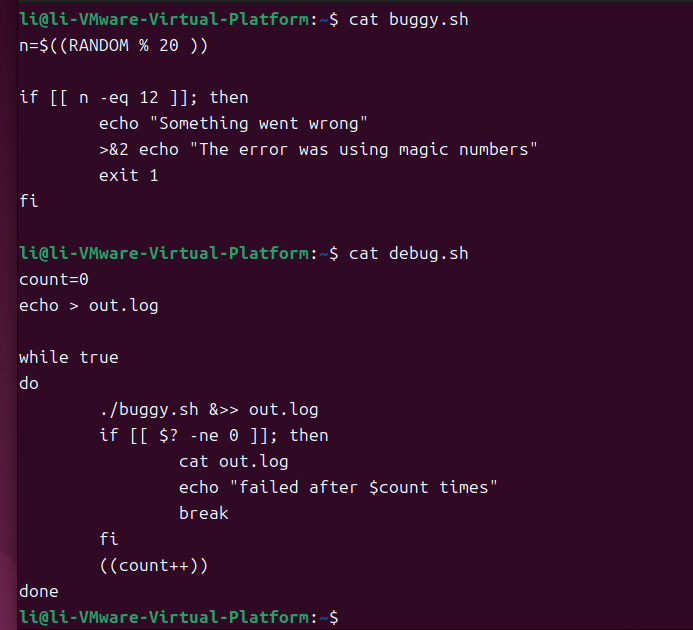
\includegraphics[width=1\textwidth]{屏幕截图 2024-09-05 143854.png}
  \caption{vim编译内容 }
    \end{figure}


\\
\newpage
     \subsection{\color{red}vim练习内容}
\noindent {\color{pink}4.下载我们提供的 vimrc,然后把它保存到 \~{}/.vimrc。 通读这个注释详细的文件 (用 Vim!), 然后观察 Vim 在这个新的设置下看起来和使用起来有哪些细微的区别。}
\vspace{-10pt}
\begin{figure}[H]
  \centering
  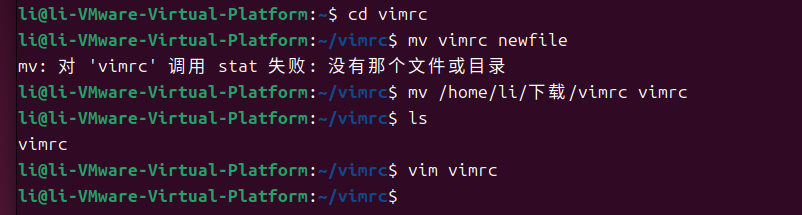
\includegraphics[width=1\textwidth]{屏幕截图 2024-09-05 165256.png}
  \caption{shell操作指令}
    \end{figure}



\begin{figure}[H]
  \centering
  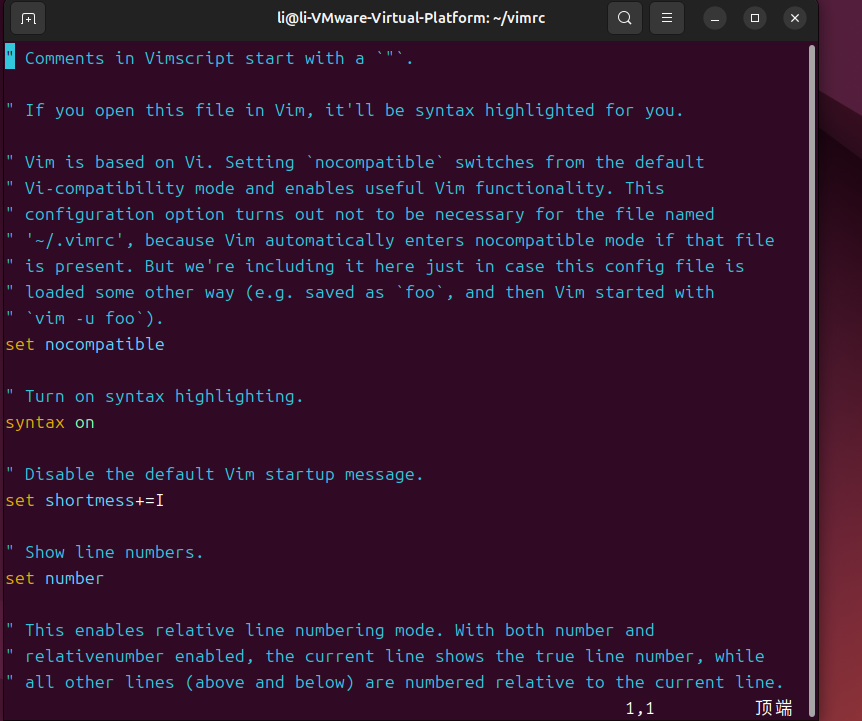
\includegraphics[width=1\textwidth]{屏幕截图 2024-09-05 165235.png}
  \caption{shell操作指令}
    \end{figure}


\noindent 5.安装和配置一个插件: ctrlp.vim.\\
\indent 5.1用 mkdir -p \~{}/.vim/pack/vendor/start 创建插件文件夹\\
\indent 5.2下载这个插件: cd \~{}/.vim/pack/vendor/start; git clone https://github.com/ctrlpvim/ctrlp.vim\\
\indent 5.3阅读这个插件的 文档。 尝试用 CtrlP 来在一个工程文件夹里定位一个文件,打开 Vim, 然后用 Vim 命令控制行开始 :CtrlP.\\
\indent 5.4自定义 CtrlP:添加 configuration 到你的 \~{}/.vimrc 来用按 Ctrl-P 打开 CtrlP\\

\begin{figure}[H]
  \centering
  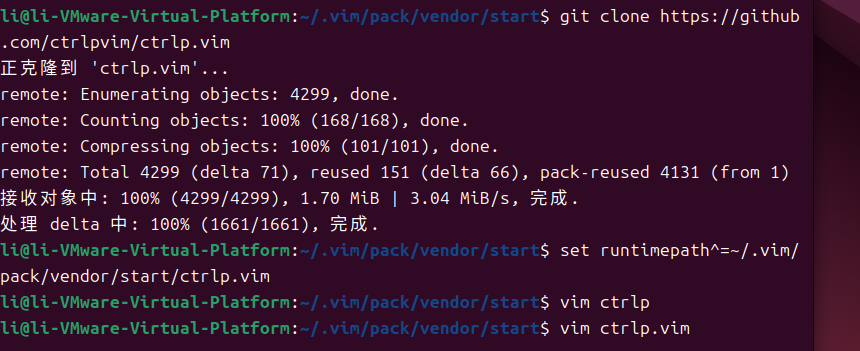
\includegraphics[width=1\textwidth]{屏幕截图 2024-09-05 170137.png}
  \caption{shell操作指令}
    \end{figure}

\begin{figure}[H]
  \centering
  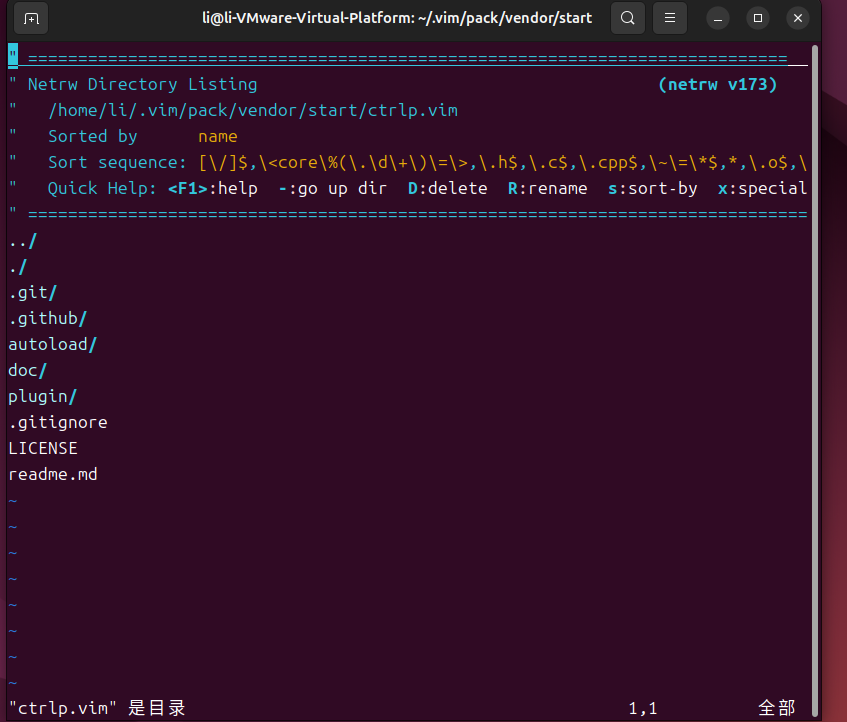
\includegraphics[width=1\textwidth]{屏幕截图 2024-09-05 165950.png}
  \caption{shell操作指令}
    \end{figure}  

    
\newpage
\subsection{{\color{red}数据整理练习内容}}

\noindent 1.统计 words 文件 (/usr/share/dict/words) 中包含至少三个 a 且不以 's 结尾的单词个数。这些单词中,出现频率前三的末尾两个字母是什么? sed 的 y 命令,或者 tr 程序也许可以帮你解决大小写的问题。共存在多少种词尾两字母组合?还有一个很 有挑战性的问题:哪个组合从未出现过?

\begin{figure}[H]
  \centering
  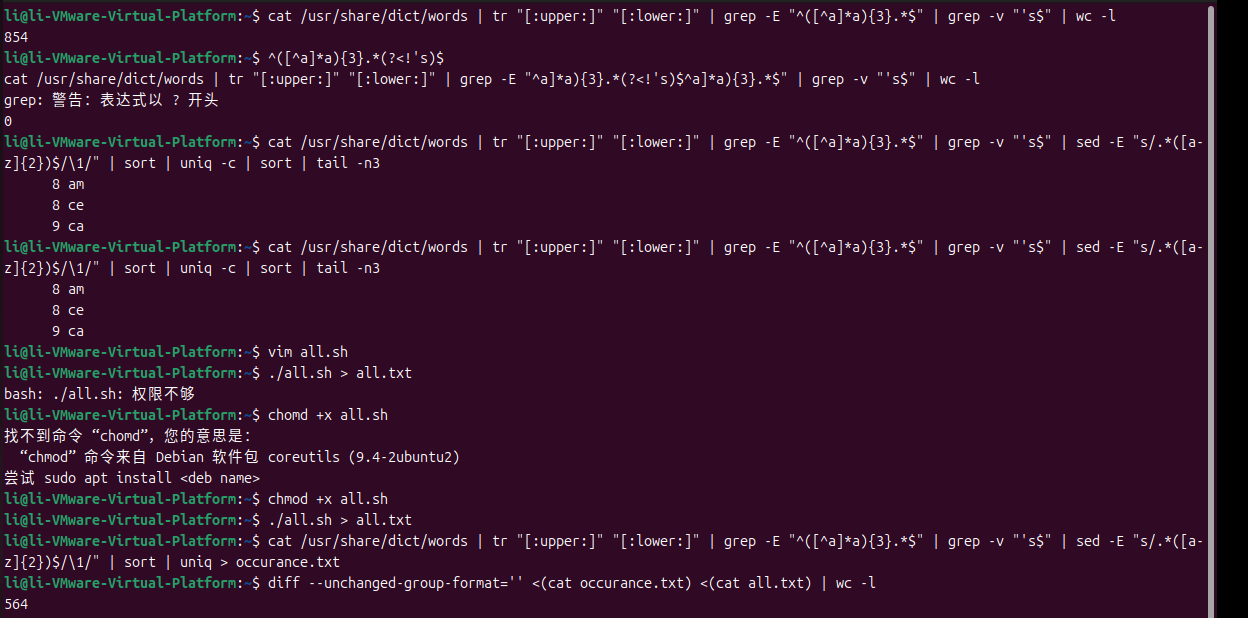
\includegraphics[width=1\textwidth]{屏幕截图 2024-09-05 235050.png}
  \caption{shell操作指令}
    \end{figure} 
\\
2.进行原地替换听上去很有诱惑力,例如: sed s/REGEX/SUBSTITUTION/ input.txt  >input.txt。但是这并不是一个明智的做法,为什么呢?还是说只有 sed 是这样的? 查看 man sed 来完成这个问题
\begin{figure}[H]
  \centering
  
\includegraphics[width=1\textwidth]{屏幕截图 2024-09-05 235124.png}
  \caption{shell操作指令}
    \end{figure} 




\section{实例大纲}
\subsection{\color{green}shell和vim实例大纲}
\begin{table}[H]
\centering
\caption{\color{red}shell与vim共用的实例展示}
\begin{tabular}{ccc} 
\toprule
\hline
 1&  for    & for循环求出1到100的和  \\ 
\hline
 2&case  & 使用case来进行选择分支 \\ 
\hline
3&$0 $1 $2 $3...  &传入参数执行文件 \\ 
\hline
4&expr $a +/- $b  &对数值进行简单的加减运算 \\ 
\hline
5&while &用while循环输出1到5 \\ 
\hline
6&case+while  &用case终止while循环 \\ 
\hline
7&创建function  &创建fun函数  \\ 
\hline
 8&echo 文字 > 文件 &定向输入并且覆盖原有文件  \\ 
\hline
9&echo 文字 >> 文件  &在文件末尾后面添加文字 \\ 
\hline
 10&date &显示当前时间  \\ 
\hline
11&-eq &判断语句的使用 \\ 
\hline
12&array  &创建并输出数组  \\ 
\hline
13&printf  &采用多种方式用printf输出   \\ 
\hline
14&shell  &传入参数执行文件  \\ 
 \hline
 15&whereis &查找命令的二进制文件、源文件及帮助文档位置  \\ 
 \hline
 16&cal  &显示日历  \\ 
 \hline
 17&env  &显示当前所有的环境变量  \\ 
 \hline
 18&mkdir  &创建一个新的目录  \\ 
 \hline
 19&rmdir &删除一个空目录  \\ 
 \hline
 20&df&显示磁盘使用空间\\
 \hline
\bottomrule
\end{tabular}
\end{table}



    


\subsection{\color{green}vim实例}
\begin{table}[H]
\centering
\caption{\color{red}vim的实例展示大纲}
\begin{tabular}{ccc} 
\toprule

\hline
 1&    :wq         &  保存然后退出                       \\ 
\hline
 2&:e {文件名}  & 打开要编辑的文件  \\ 
\hline
 3&:ls  &   显示打开的缓存\\ 
\hline
 4& Ctrl+v & 可视化块  \\ 
\hline
 5& x & 删除字符  \\ 
\hline
 6& jj$i &   插入文字到行尾\\
 \hline

 7& jj. &   重复第二个打印\\
 \hline
8 &:s &   (替换)命令\\
 \hline
9 & ci( &   改变当前括号内的内容\\
 \hline
 10 & :sp / :vsp &   分割窗口\\
 \hline
\bottomrule
\end{tabular}
\end{table}


\subsection{\color{green}数据整理实例大纲}
\begin{table}[H]
\centering
\caption{\color{red}数据整理的实例展示}
\begin{tabular}{ccc} 
\toprule

\hline
 1&    tr "[:upper:]" "[:lower:]"       &  大小写转换                       \\ 
\hline
 2&^([^a]*a){3}.*[^'s]$  & 查找一个以 a 结尾的字符串三次 \\ 
\hline
 3&grep -v "\'s$" &   匹配结尾为’s 的结果,然后取反\\ 
\hline
 4& --unchanged-group-format='' &两个文件中相同的内容设置为空字符串 \\ 
\hline
 5&sed -i.bak s/REGEX/SUBSTITUTION/ input.txt & 自动创建一个后缀为 .bak 的备份文件  \\ 
\hline

\bottomrule
\end{tabular}
\end{table}


\newpage

\section{shell与vim的实例展示}

{\color{red}用vim编译,然后用cat查看文件内容,再用bash运行程序。}
\\
\\
1.for循环求出1到100的和。
\begin{figure}[H]
  \centering
  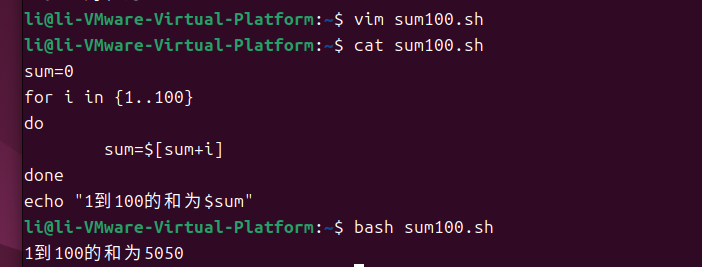
\includegraphics[width=1\textwidth]{屏幕截图 2024-08-31 120440.png}
  \caption{for循环}
    \end{figure}


2.使用case来进行选择分支。
\begin{figure}[H]
  \centering
  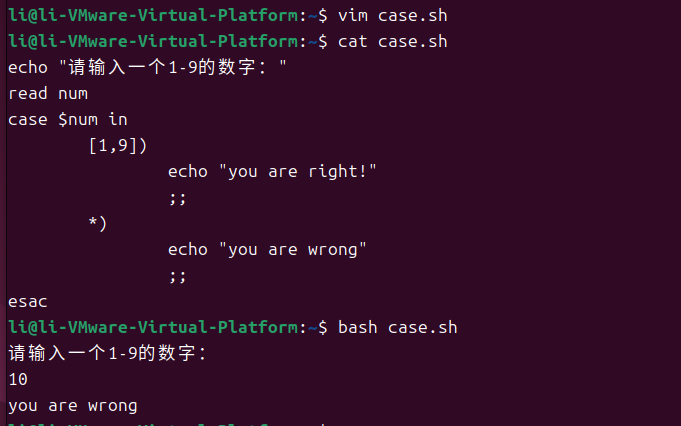
\includegraphics[width=1\textwidth]{屏幕截图 2024-08-31 120922.png}
  \caption{case示例}
    \end{figure}
\\

3.传入参数执行文件。
\begin{figure}[H]
  \centering
  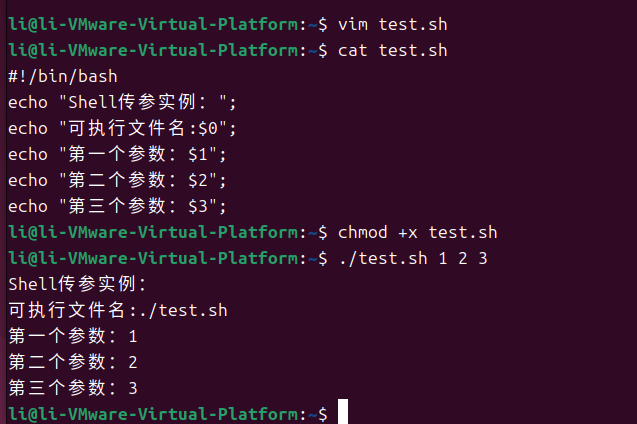
\includegraphics[width=1\textwidth]{屏幕截图 2024-08-31 194338.png}
  \caption{shell传参实例}
\end{figure}

4.对数值进行简单的加减运算。
\begin{figure}[H]
  \centering
  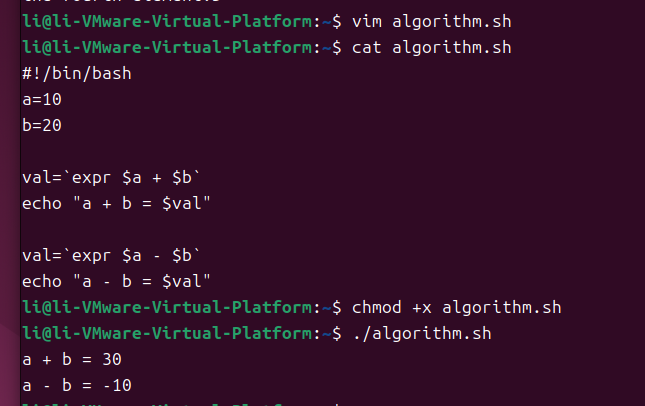
\includegraphics[width=1\textwidth]{屏幕截图 2024-08-31 200646.png}
  \caption{基本运算}
    \end{figure}

5.用while循环输出1到5。
\begin{figure}[H]
  \centering
  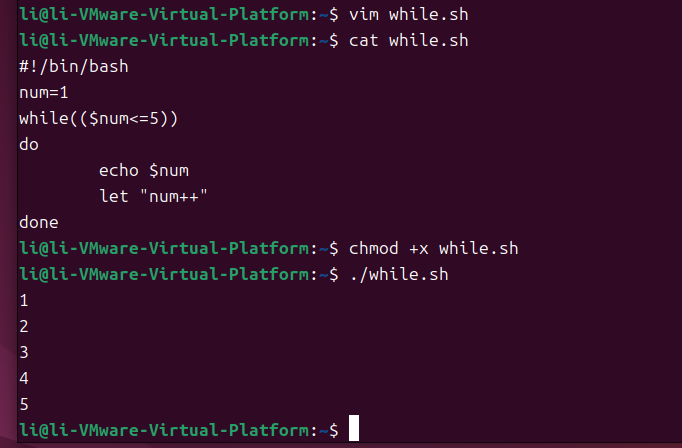
\includegraphics[width=1\textwidth]{屏幕截图 2024-09-01 205922.png}
  \caption{while循环}
    \end{figure}

6.用case终止while循环。
\begin{figure}[H]
  \centering
  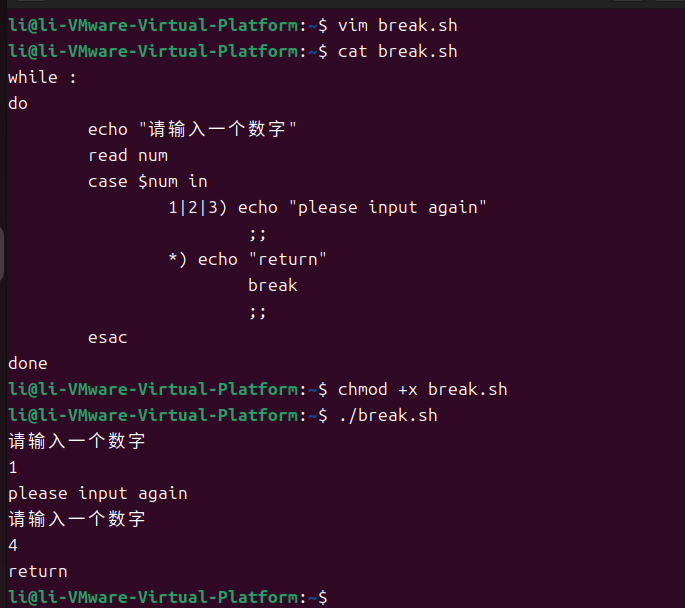
\includegraphics[width=1\textwidth]{屏幕截图 2024-09-01 210447.png}
  \caption{while+case判断}
    \end{figure}
\newpage
7.创建fun函数
\begin{figure}[H]
  \centering
  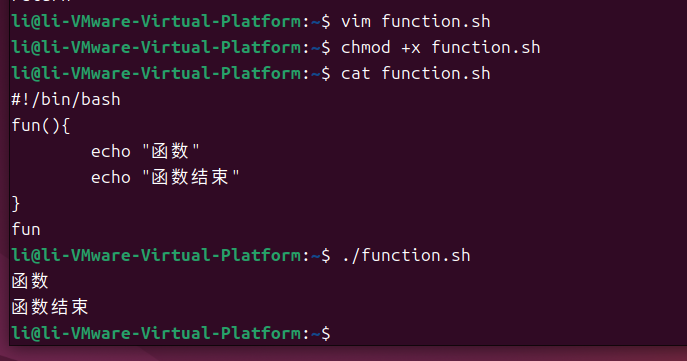
\includegraphics[width=1\textwidth]{屏幕截图 2024-09-01 233555.png}
  \caption{创建函数}
    \end{figure}

8.定向输入并且覆盖原有文件
\begin{figure}[H]
  \centering
  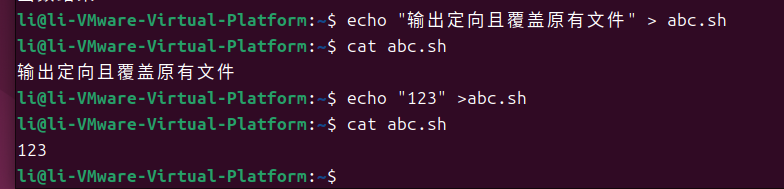
\includegraphics[width=1\textwidth]{屏幕截图 2024-09-01 233829.png}
  \caption{覆盖输入}
    \end{figure}

9.在文件末尾后面添加文字。
\begin{figure}[H]
  \centering
  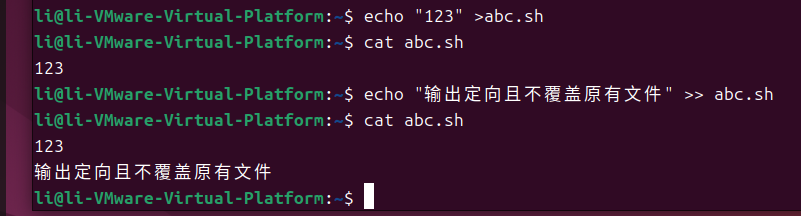
\includegraphics[width=1\textwidth]{屏幕截图 2024-09-01 233917.png}
  \caption{不覆盖输入}
    \end{figure}


10.显示当前时间。
\begin{figure}[H]
  \centering
  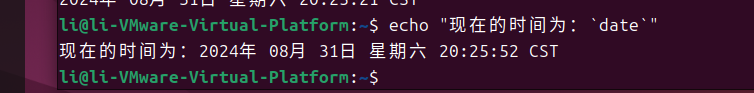
\includegraphics[width=1\textwidth]{屏幕截图 2024-08-31 202609.png}
  \caption{显示时间}
    \end{figure}

11.判断语句的使用。
\begin{figure}[H]
  \centering
  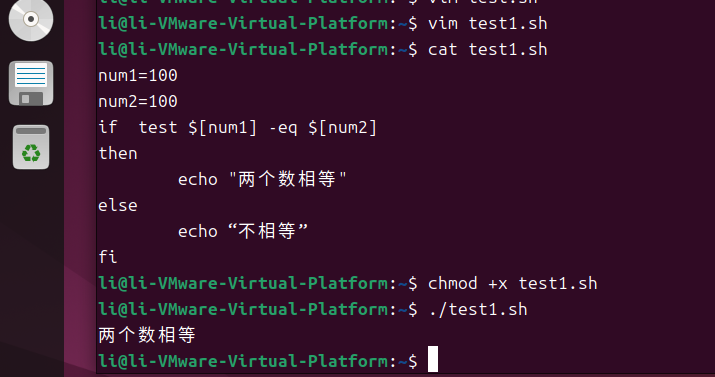
\includegraphics[width=1\textwidth]{屏幕截图 2024-09-01 205629.png}
  \caption{判断语句}
    \end{figure}
\newpage
12.创建并输出数组。
\begin{figure}[H]
  \centering
  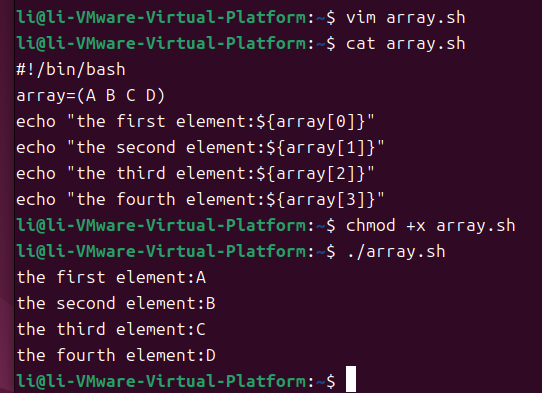
\includegraphics[width=1\textwidth]{屏幕截图 2024-08-31 195429.png}
  \caption{数组}
    \end{figure}

13.采用多种方式用printf输出
\begin{figure}[H]
  \centering
  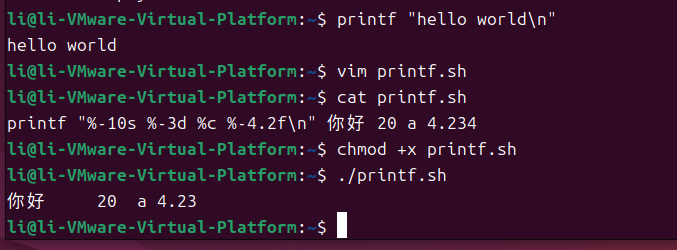
\includegraphics[width=1\textwidth]{屏幕截图 2024-08-31 204133.png}
  \caption{printf输出}
    \end{figure}

\newpage
14.传入参数执行文件。
\begin{figure}[H]
  \centering
  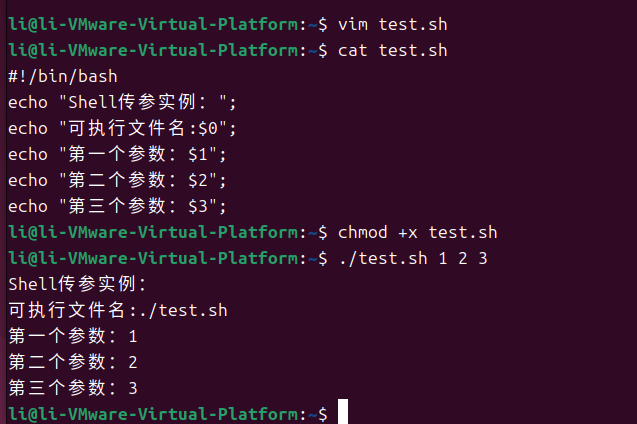
\includegraphics[width=1\textwidth]{屏幕截图 2024-08-31 194338.png}
  \caption{shell传参实例}
\end{figure}

15.查找命令的二进制文件、源文件及帮助文档位置
 \begin{figure}[H]
  \centering
  
\includegraphics[width=1\textwidth]{屏幕截图 2024-09-05 230933.png}
  \caption{whereis}
    \end{figure}
    \newpage
16.显示日历
\begin{figure}[H]
  \centering
  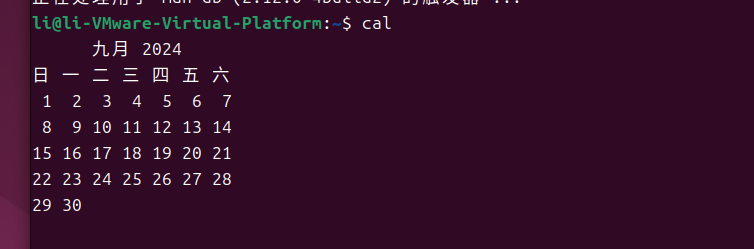
\includegraphics[width=1\textwidth]{屏幕截图 2024-09-05 231209.png}
  \caption{cal}
    \end{figure}

17.显示当前所有的环境变量
\begin{figure}[H]
  \centering
  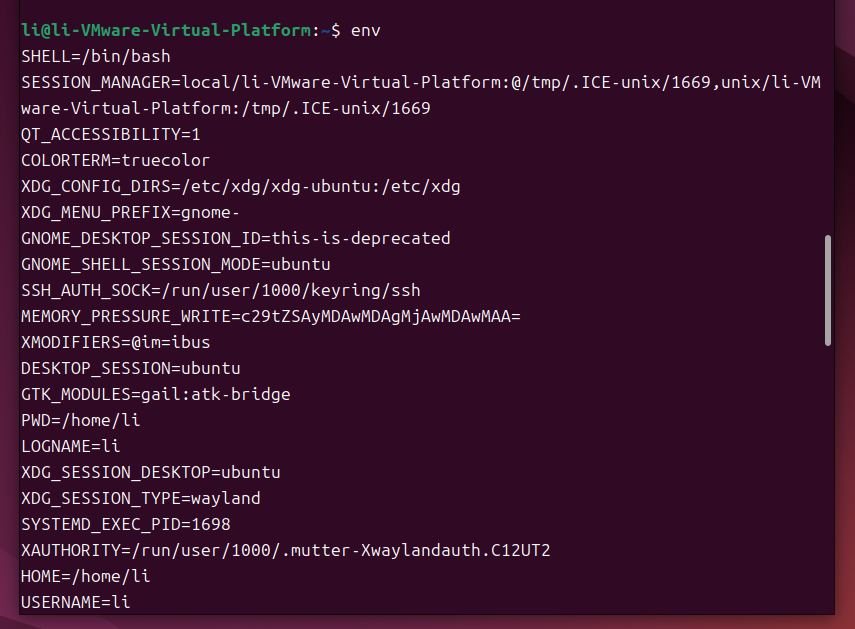
\includegraphics[width=1\textwidth]{屏幕截图 2024-09-05 231711.png}
  \caption{env}
    \end{figure}

    \newpage
18.创建一个新的目录 
   \begin{figure}[H]
  \centering
  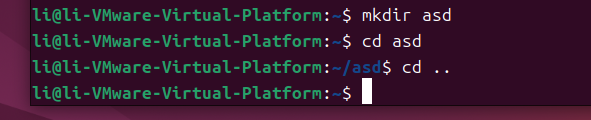
\includegraphics[width=1\textwidth]{屏幕截图 2024-09-05 232120.png}
  \caption{mkdir }
    \end{figure}
19.删除一个空目录
   \begin{figure}[H]
  \centering
  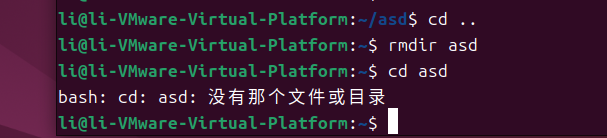
\includegraphics[width=1\textwidth]{屏幕截图 2024-09-05 232156.png}
  \caption{rmdir}
    \end{figure}
    
20.显示磁盘使用空间
    \begin{figure}[H]
  \centering
  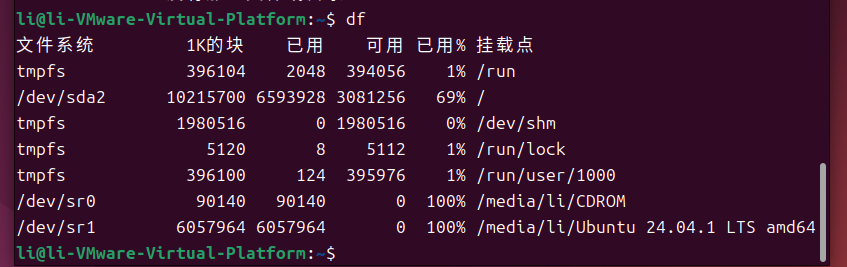
\includegraphics[width=1\textwidth]{屏幕截图 2024-09-05 232224.png}
  \caption{df}
    \end{figure}

   
\newpage
\section{个人心得}
\\
我认为使用Shell脚本的最大优势在于其强大而灵活的系统控制能力,尤其在Unix和Linux系统上表现突出。它提供了一种简洁易用的方式,能够将复杂的系统任务如文件处理、网络管理、系统维护自动化。Shell脚本几乎都是系统命令的组合,简单易学,特别适合小型任务,如批量处理文件或执行系统管理任务,并且具备良好的跨平台兼容性。
\\
\indent 然而,Shell脚本的可读性和维护性是一个值得关注的方面。编写时应注重使用有意义的变量名、结构化代码、以及详细的注释,尤其在复杂的逻辑处理中,这可以帮助后续维护和理解。同时,Shell脚本的调试相对较弱,建议在脚本中加入错误处理和日志记录,使用set -e和trap等命令,避免因简单错误导致脚本崩溃。
\\
\indent 对于性能优化,Shell脚本在处理复杂或大规模任务时,可能表现不如其他编程语言高效。为此,尽量使用内建命令,如awk、sed、grep,并减少不必要的外部命令调用和文件读写。Shell脚本在系统管理、批量操作、自动化部署等场景中表现优秀,但在性能要求高的复杂任务中,建议结合其他语言使用。
\\

\section{github网址}
\href{https://github.com/newbeginnerlzh/git-task01.git}{\color{red}https://github.com/newbeginnerlzh/git-task01.git}

\end{document}


